\documentclass{ximera}
% \input{../../xmpreamble.tex}

\title{Vector Arithmetic}
\author{Zack Reed}

\begin{document}
\begin{abstract}
In this activity we continue our grounded exploration of vectors, focusing on vector arithmetic: addition, scaling, and magnitude.
\end{abstract}
\maketitle

\section*{Vector Arithmetic}

\subsection*{Vector Addition}

Now we extend the idea of vector addition.

\begin{center}
    \youtube{jjxtIx7XkoA}
\end{center}

\begin{problem}
(Reference the end of the video to answer the following question.)
Which of the following best describes the new velocity of the kids holding on to their box? (Just guess for now, based on your intuition.)
\begin{multipleChoice}
    \choice{The new velocity orients upwards and to the right.}
    \choice[correct]{The new velocity orients directly upwards.}
    \choice{The new velocity orients upwards and to the left.}
    \choice{The boys and box stop moving.}
\end{multipleChoice}
\begin{feedback}
Think about moving along one vector, and then moving along the other vector starting from the end of the first vector.
(insert video)
\end{feedback}
\end{problem}


\begin{problem}
    Let's practice adding and subtracting vectors component-wise. Compute the following vector sums and differences:
    \begin{enumerate}
        \item If $\vec{v}=[3,4]$ and $\vec{u}=[1,2]$, then $\vec{v}+\vec{u}=[\answer{4},\answer{6}]$
        \item If $\vec{v}=[-2,5]$ and $\vec{u}=[1,-2]$, then $\vec{v}-\vec{u}=[\answer{-3},\answer{7}]$
        \item If $\vec{v}=[0,7]$ and $\vec{u}=[5,-3]$, then $\vec{v}+\vec{u}=[\answer{5},\answer{4}]$
        \item If $\vec{v}=[1,2,3]$ and $\vec{u}=[4,5,6]$, then $\vec{v}+\vec{u}=[\answer{5},\answer{7},\answer{9}]$
        \item If $\vec{v}=[-1,0,2]$ and $\vec{u}=[3,-4,1]$, then $\vec{v}-\vec{u}=[\answer{-4},\answer{4},\answer{1}]$
        \item If $\vec{v}=[2,-3,5]$ and $\vec{u}=[-2,3,-5]$, then $\vec{v}+\vec{u}=[\answer{0},\answer{0},\answer{0}]$
    \end{enumerate}
    
 // ...existing code...
    \begin{feedback}
        Remember that vector addition and subtraction work component-wise. For $\vec{v}=[v_1,v_2]$ and $\vec{u}=[u_1,u_2]$, we have $\vec{v}+\vec{u}=[v_1+u_1,v_2+u_2]$ and $\vec{v}-\vec{u}=[v_1-u_1,v_2-u_2]$. This extends naturally to three dimensions!
    \end{feedback}
\end{problem}


\begin{problem}
    Now let's visualize these vector operations using the tip-to-tail method. For each vector operation, select all the diagrams that correctly represent the operation.
    
    \begin{enumerate}
        \item For $\vec{v}=[2,4]$ and $\vec{u}=[3,2]$, select all correct visualizations of the way to build $\vec{v}+\vec{u}$ from $\vec{v}$ and $\vec{u}$:
        \begin{selectAll}
            \choice{
                \begin{tikzpicture}[scale=0.75, thick, >=stealth]
                    \draw[->] (0,0) -- (2,4) node[midway,left] {$\vec{v}$};
                    \draw[->] (2,4) -- (4,8) node[midway,left] {$\vec{v}$};
                    \draw[->] (4,8) -- (7,10) node[midway,right] {$\vec{u}$};
                    \draw[->,thick,blue] (0,0) -- (7,10) node[midway,below right] {$\vec{v}+\vec{u}$};
                    \draw[gray,dashed] (-0.5,0) -- (8,0);
                    \draw[gray,dashed] (0,-0.5) -- (0,11);
                \end{tikzpicture}
            }
            \choice[correct]{
                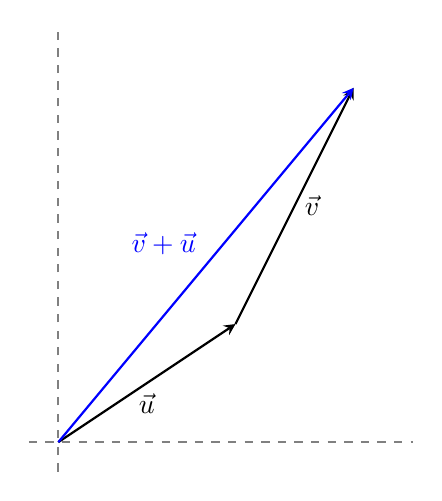
\begin{tikzpicture}[scale=0.75, thick, >=stealth]
                    \draw[->] (0,0) -- (3,2) node[midway,below] {$\vec{u}$};
                    \draw[->] (3,2) -- (5,6) node[midway,right] {$\vec{v}$};
                    \draw[->,thick,blue] (0,0) -- (5,6) node[midway,above left] {$\vec{v}+\vec{u}$};
                    \draw[gray,dashed] (-0.5,0) -- (6,0);
                    \draw[gray,dashed] (0,-0.5) -- (0,7);
                \end{tikzpicture}
            }
            \choice[correct]{
                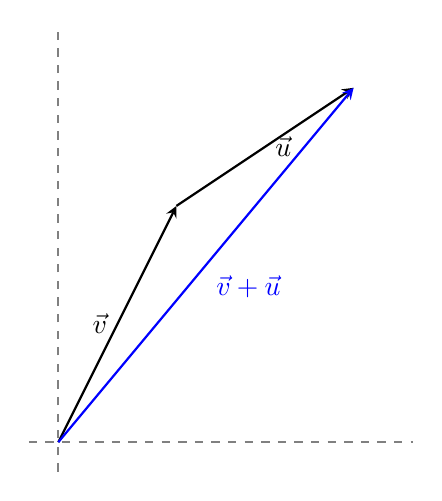
\begin{tikzpicture}[scale=0.75, thick, >=stealth]
                    \draw[->] (0,0) -- (2,4) node[midway,left] {$\vec{v}$};
                    \draw[->] (2,4) -- (5,6) node[midway,right] {$\vec{u}$};
                    \draw[->,thick,blue] (0,0) -- (5,6) node[midway,below right] {$\vec{v}+\vec{u}$};
                    \draw[gray,dashed] (-0.5,0) -- (6,0);
                    \draw[gray,dashed] (0,-0.5) -- (0,7);
                \end{tikzpicture}
            }
            \choice{
                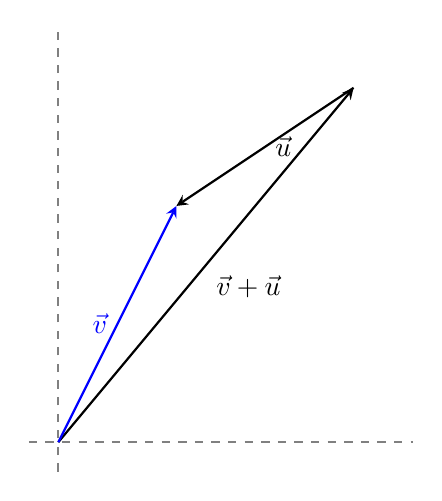
\begin{tikzpicture}[scale=0.75, thick, >=stealth]
                    \draw[->] (0,0) -- (5,6) node[midway,below right] {$\vec{v}+\vec{u}$};
                    \draw[->] (5,6) -- (2,4) node[midway,right] {$\vec{u}$};
                    \draw[->,thick,blue] (0,0) -- (2,4) node[midway,left] {$\vec{v}$};
                    \draw[gray,dashed] (-0.5,0) -- (6,0);
                    \draw[gray,dashed] (0,-0.5) -- (0,7);
                \end{tikzpicture}
            }
        \end{selectAll}

        \item For $\vec{v}=[1,6]$ and $\vec{u}=[5,-2]$, select all correct visualizations of the way to build $\vec{v}+\vec{u}$ from $\vec{v}$ and $\vec{u}$:
        \begin{selectAll}
            \choice{
                \begin{tikzpicture}[scale=0.75, thick, >=stealth]
                    \draw[->] (0,0) -- (6,4) node[midway,above left] {$\vec{v}+\vec{u}$};
                    \draw[->] (6,4) -- (1,6) node[midway,right] {$\vec{u}$};
                    \draw[->,thick,blue] (0,0) -- (1,6) node[midway,left] {$\vec{v}$};
                    \draw[gray,dashed] (-1,0) -- (7,0);
                    \draw[gray,dashed] (0,-3) -- (0,13);
                \end{tikzpicture}
            }
            \choice[correct]{
                \begin{tikzpicture}[scale=0.75, thick, >=stealth]
                    \draw[->] (0,0) -- (5,-2) node[midway,below] {$\vec{u}$};
                    \draw[->] (5,-2) -- (6,4) node[midway,right] {$\vec{v}$};
                    \draw[->,thick,blue] (0,0) -- (6,4) node[midway,above left] {$\vec{v}+\vec{u}$};
                    \draw[gray,dashed] (-1,0) -- (7,0);
                    \draw[gray,dashed] (0,-3) -- (0,13);
                \end{tikzpicture}
            }
            \choice{
                \begin{tikzpicture}[scale=0.75, thick, >=stealth]
                    \draw[->] (0,0) -- (1,6) node[midway,left] {$\vec{v}$};
                    \draw[->] (1,6) -- (2,12) node[midway,left] {$\vec{v}$};
                    \draw[->] (2,12) -- (7,10) node[midway,above right] {$\vec{u}$};
                    \draw[->,thick,blue] (0,0) -- (7,10) node[midway,below right] {$\vec{v}+\vec{u}$};
                    \draw[gray,dashed] (-1,0) -- (8,0);
                    \draw[gray,dashed] (0,-3) -- (0,13);
                \end{tikzpicture}
            }
            \choice[correct]{
                \begin{tikzpicture}[scale=0.75, thick, >=stealth]
                    \draw[->] (0,0) -- (1,6) node[midway,left] {$\vec{v}$};
                    \draw[->] (1,6) -- (6,4) node[midway,above right] {$\vec{u}$};
                    \draw[->,thick,blue] (0,0) -- (6,4) node[midway,below right] {$\vec{v}+\vec{u}$};
                    \draw[gray,dashed] (-1,0) -- (7,0);
                    \draw[gray,dashed] (0,-3) -- (0,13);
                \end{tikzpicture}
            }
        \end{selectAll}
    \end{enumerate}
    
    \begin{feedback}
        Remember the tip-to-tail method: place the tail of the second vector at the tip of the first vector. The sum is the vector from the tail of the first to the tip of the second. For subtraction $\vec{v}-\vec{u}$, think of it as $\vec{v}+(-\vec{u})$, where $-\vec{u}$ points in the opposite direction of $\vec{u}$.
    \end{feedback}
\end{problem}

\subsection*{Scaling Vectors}

Now let's use the context of momentum to learn about scaling vectors.

(insert video)

\begin{problem}
    (Reference the end of the video to answer the following question.)
    
    If Riley and Taylor have a combined mass of $150$N, and the box has a mass of $200$N, with velocity vectors $\vec{v}_{RT}=[-5,2]$ and $\vec{v}_B=[5,2]$, in which direction will the box and boys move togetehr after the collision?
    \begin{multipleChoice}
        \choice{They will move to the left and upwards.}
        \choice[correct]{They will move directly upwards.}
        \choice{They will move to the right and upwards.}
        \choice{They will stop moving.}
    \end{multipleChoice}
    \begin{feedback}
        Remember that momentum is mass times velocity. The box has more mass than the boys, so it will have a greater influence on the direction of their combined motion, even though the direction vectors have the same length but point in opposite horizontal directions.
        (insert video)
    \end{feedback}
\end{problem}

\begin{definition}
The more formal way to talk about adding and scaling vectors is the idea of \emph{linear combinations}. 

That is, a linear combination of vectors $\vec{u}$ and $\vec{v}$ adds together scaled versions of the vectors. For scalars $r$ and $s$, the linear combination of $\vec{u}$ and $\vec{v}$ is given by $r\vec{u}+s\vec{v}$.
\end{definition}

\begin{remark}
    Both vector addition and scalar multiplication can be done component-wise. That is, if $\vec{u}=[u_1,u_2]$ and $\vec{v}=[v_1,v_2]$, then
    \[\vec{u}+\vec{v}=[u_1+v_1,u_2+v_2]\]
    and for a scalar $r$,
    \[r\vec{u}=[ru_1,ru_2].\]
\end{remark}

\begin{problem}
    Let's try out computing a few linear combinations of vectors. Compute the following:
    \begin{enumerate}
        \item $2[3,4]+3[1,2]=[\answer{15},\answer{20}]$
        \item $-1[2,5]+4[-1,1]=[\answer{-6},\answer{-1}]$
        \item $3[0,2]+2[3,0]=[\answer{6},\answer{6}]$
        \item $-2[1,1]+0.5[4,6]=[\answer{0},\answer{2}]$
        \item $0[5,7]+3[-2,4]=[\answer{-6},\answer{12}]$
    \end{enumerate}

    \begin{feedback}
        A simple comprehensive formula for a linear combination of two vectors is $r[u_1,u_2]+s[v_1,v_2]=[ru_1+sv_1,ru_2+sv_2]$, though we don't recommend memorizing a formula, think about why it works the way it does and remember the general idea. This special formula only works for two 2-dimensional vectors.
    \end{feedback}
\end{problem}

\begin{problem}
    Now, write out the arithmetic formula that creates the following vector sums.

    \begin{expandable}{stuff}{Hint for negative numbers}
        Negative scalars reverse the direction of the vector.
    \end{expandable}
    
    \begin{enumerate}
        \item 
        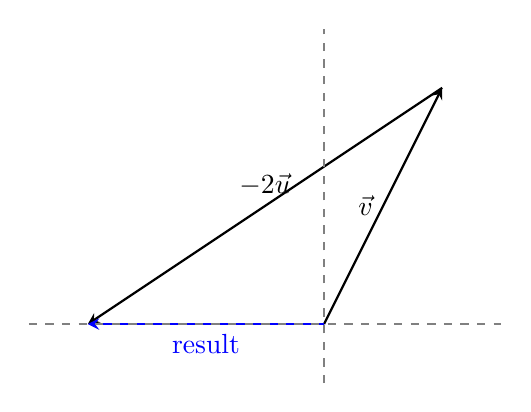
\begin{tikzpicture}[scale=0.75, thick, >=stealth]
            \draw[->] (0,0) -- (2,4) node[midway,left] {$\vec{v}$};
            \draw[->] (2,4) -- (-4,0) node[midway,above] {$-2\vec{u}$};
            \draw[->,thick,blue] (0,0) -- (-4,0) node[midway,below] {result};
            \draw[gray,dashed] (-5,0) -- (3,0);
            \draw[gray,dashed] (0,-1) -- (0,5);
        \end{tikzpicture}
        
        This figure represents the vector sum $\answer{1}\vec{v}+\answer{-2}\vec{u}$.
        
        \item 
        \begin{tikzpicture}[scale=0.75, thick, >=stealth]
            \draw[->] (0,0) -- (6,3) node[midway,below] {$2\vec{v}$};
            \draw[->] (6,3) -- (8,4) node[midway,above right] {$\vec{u}$};
            \draw[->,thick,blue] (0,0) -- (8,4) node[midway,above left] {result};
            \draw[gray,dashed] (-1,0) -- (9,0);
            \draw[gray,dashed] (0,-1) -- (0,5);
        \end{tikzpicture}
        
        This figure represents the vector sum $\answer{2}\vec{v}+\answer{1}\vec{u}$.
        
        \item 
        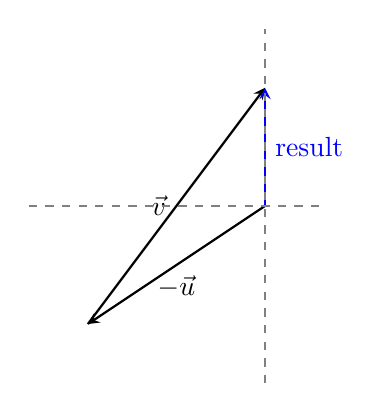
\begin{tikzpicture}[scale=0.75, thick, >=stealth]
            \draw[->] (0,0) -- (-3,-2) node[midway,below] {$-\vec{u}$};
            \draw[->] (-3,-2) -- (0,2) node[midway,left] {$\vec{v}$};
            \draw[->,thick,blue] (0,0) -- (0,2) node[midway,right] {result};
            \draw[gray,dashed] (-4,0) -- (1,0);
            \draw[gray,dashed] (0,-3) -- (0,3);
        \end{tikzpicture}
        
        This figure represents the vector sum $\answer{1}\vec{v}+\answer{-1}\vec{u}$.
        
        \item 
        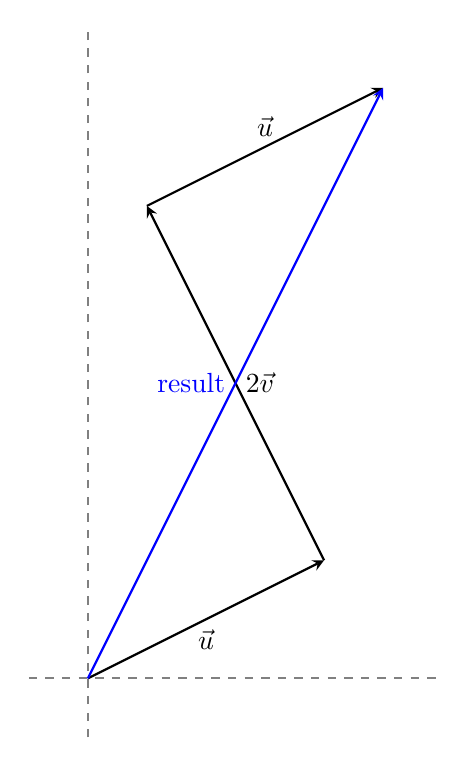
\begin{tikzpicture}[scale=0.75, thick, >=stealth]
            \draw[->] (0,0) -- (4,2) node[midway,below] {$\vec{u}$};
            \draw[->] (4,2) -- (1,8) node[midway,right] {$2\vec{v}$};
            \draw[->] (1,8) -- (5,10) node[midway,above] {$\vec{u}$};
            \draw[->,thick,blue] (0,0) -- (5,10) node[midway,left] {result};
            \draw[gray,dashed] (-1,0) -- (6,0);
            \draw[gray,dashed] (0,-1) -- (0,11);
        \end{tikzpicture}
        
        This figure represents the vector sum $\answer{1}\vec{u}+\answer{2}\vec{v}+\answer{1}\vec{u}$.
    \end{enumerate}
    
    \begin{feedback}
        Remember that vector addition works by following one of the vectors, then following the next vector starting from the tip of the first vector, and continuing until you've followed all vectors in the sum. 

        Also remember that multiplying a vector by a number scales the vector, and multiplying by a negative number reverses the vector's direction.
    \end{feedback}
\end{problem}


\subsection*{Magnitude and Direction of Vectors}

While a guiding intuition so far has been that we care about \emph{how big} a vector is and \emph{in what direction} it points, we haven't yet made these ideas precise. Let's use the context of expended energy (work) to explore these ideas.

(insert video)

\begin{problem}
    (Reference the end of the video to answer the following question.)
    
    How long is the vector $\vec{D}=[-100,40]$? 

    \begin{selectAll}
    \choice[correct]{$||\vec{D}||=\sqrt{(-100)^2+40^2}$}
    \choice[correct]{$||\vec{D}||=\sqrt{11600}$}
    \choice{$||\vec{D}||=100+40$}
    \choice{$||\vec{D}||=140$}
    \end{selectAll}
    \begin{feedback}
        The length of a vector $\vec{v}=[v_1,v_2]$ is given by the Pythagorean Theorem applied to the vector and its components: $||\vec{v}||=\sqrt{v_1^2+v_2^2}$.
    \end{feedback}
\end{problem}

Let's break down how vector magnitudes (denoted $||\vec{v}||$) are computed and thought of.

(video)

\begin{problem}
    (Reference the end of the video to answer the following question.)

    How much force is applied by the vector $\vec{F}=[-20,8]$?

    $\vec{F}$ applies a force of $\answer{\sqrt{(-20)^2+8^2}}$ Newtons.

    \begin{feedback}
        Even though force doesn't have a physical length, we still use the vector length to tell us the amount of force applied (the magnitude).
    \end{feedback}
\end{problem}

Now we put it all together to compute the energy spent (work) in this ideal case where the force and displacement are in the same direction.

(video)

\begin{problem}
    (Reference the end of the video to answer the following question.)

    Riley and Taylor push a box with a force of $\vec{F}=[-20,8]$ Newtons over a displacement of $\vec{D}=[-100,40]$ meters. How much work (i.e. energy spent) do they do on the box?

    They do 

    \begin{multipleChoice}
        \choice{$W=||\vec{F}||+||\vec{D}||$ Joules of work.}
        \choice{$W=||\vec{F}||-||\vec{D}||$ Joules of work.}
        \choice[correct]{$W=||\vec{F}||\cdot||\vec{D}||$ Joules of work.}
        \choice[correct]{$W=2320$ Joules of work.}
        \choice{$W=\sqrt{12064}$ Joules of work.}
    \end{multipleChoice}

    \begin{feedback}
        In this ideal case, the work done is given by $W=||\vec{F}||\cdot||\vec{D}||$.
    \end{feedback}

\end{problem}

We assumed that the force and displacement were in the same direction. Is this assumption valid? What might we check to see if the force and displacement are truly in the same direction?

(video)

\begin{problem}
    (Reference the end of the video to answer the following question.)

    The force vector $\vec{F}=[-20,8]$ and the displacement vector $\vec{D}=[-100,40]$ \wordChoice{
        \choice{are not in the same direction}
        \choice[correct]{are in the same direction}
} because \wordChoice{
        \choice{they do not share a direction vector.}
        \choice[correct]{they share direction vectors.}
}
\end{problem}


\end{document}